% Section content template for individual Educative lessons
% This file contains the actual content for a specific section
% Generated from Educative API section content

% Section: Design of a Rate Limiter
% Section ID: 5287353329647616
% Section Slug: design-of-a-rate-limiter
% Generated: 2025-12-07T21:29:56.772747

\subsection{High-level design}\label{wHkZt5WUNjizQMU7gVHWM}
\\
A rate limiter can be deployed as a separate service that will interact with a web server, as shown in the figure below. When a request is received, the rate limiter suggests whether the request should be forwarded to the server or not. The rate limiter consists of rules that should be followed by each incoming request. These rules define the throttling limit for each operation. Let 's go through a rate limiter rule from \href{https://github.com/envoyproxy/ratelimit}{Lyft}, which has open-sourced its rate limiting component.

\textbf{Rate-limiting rules from Lyft}
\newpage
\begin{lstlisting}[language=Python]
domain: messaging
descriptors:
   -key: message_type
    value: marketing
    rate_limit:
               unit: day
               request_per_unit: 5
\end{lstlisting}

In the above rate-limiting rule, the \texttt{unit} is set to \texttt{day} and the request\_per\_unit is set to \texttt{5}. These parameters define that the system can allow five marketing messages per day.

\begin{figure}[htbp]
 \centering
 \begin{subfigure}[b]{0.48\textwidth}
 \centering
 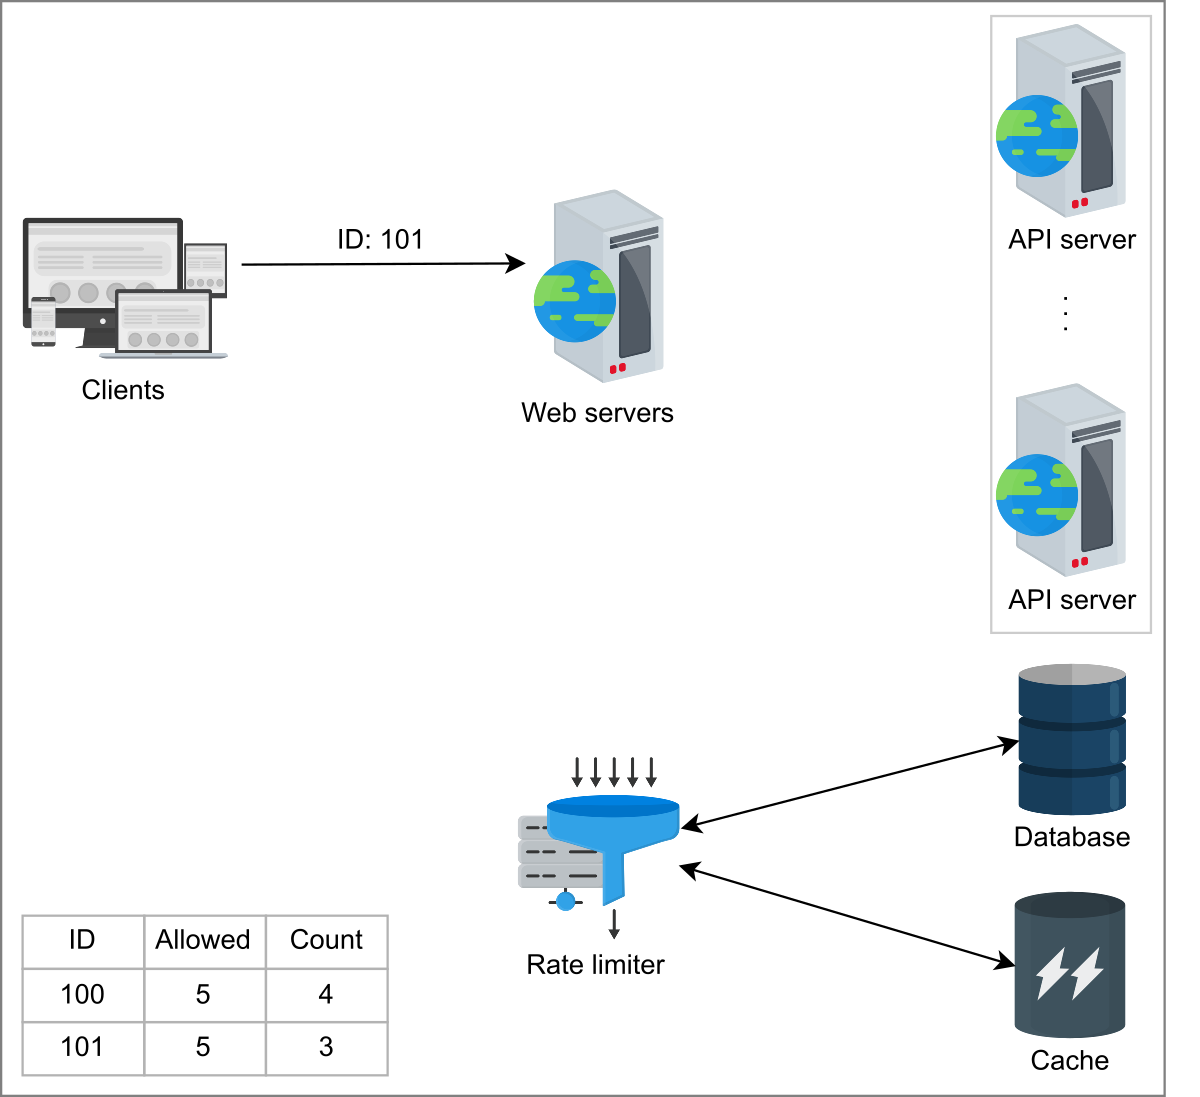
\includegraphics[width=\textwidth]{Images/chapter_19/section_5287353329647616/6576151204200448.png}
 \caption{A request with ID 101, received by one of the web servers}
 \end{subfigure}
 \hfill
 \begin{subfigure}[b]{0.48\textwidth}
 \centering
 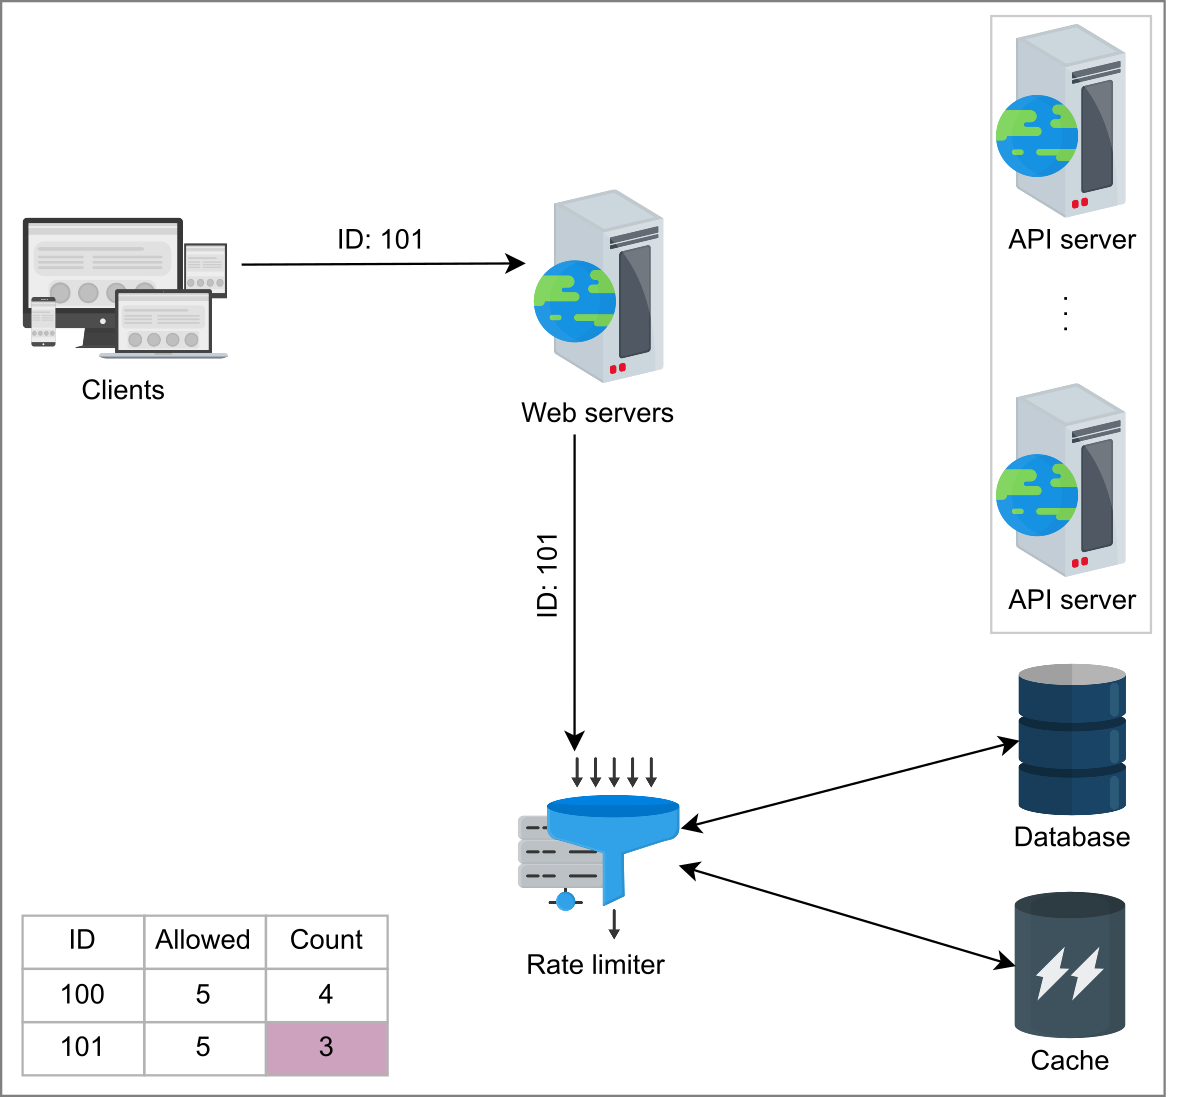
\includegraphics[width=\textwidth]{Images/chapter_19/section_5287353329647616/4553178624557056.png}
 \caption{The request is forwarded to the rate limiter}
 \end{subfigure}
\end{figure}

\begin{figure}[htbp]
 \centering
 \begin{subfigure}[b]{0.48\textwidth}
 \centering
 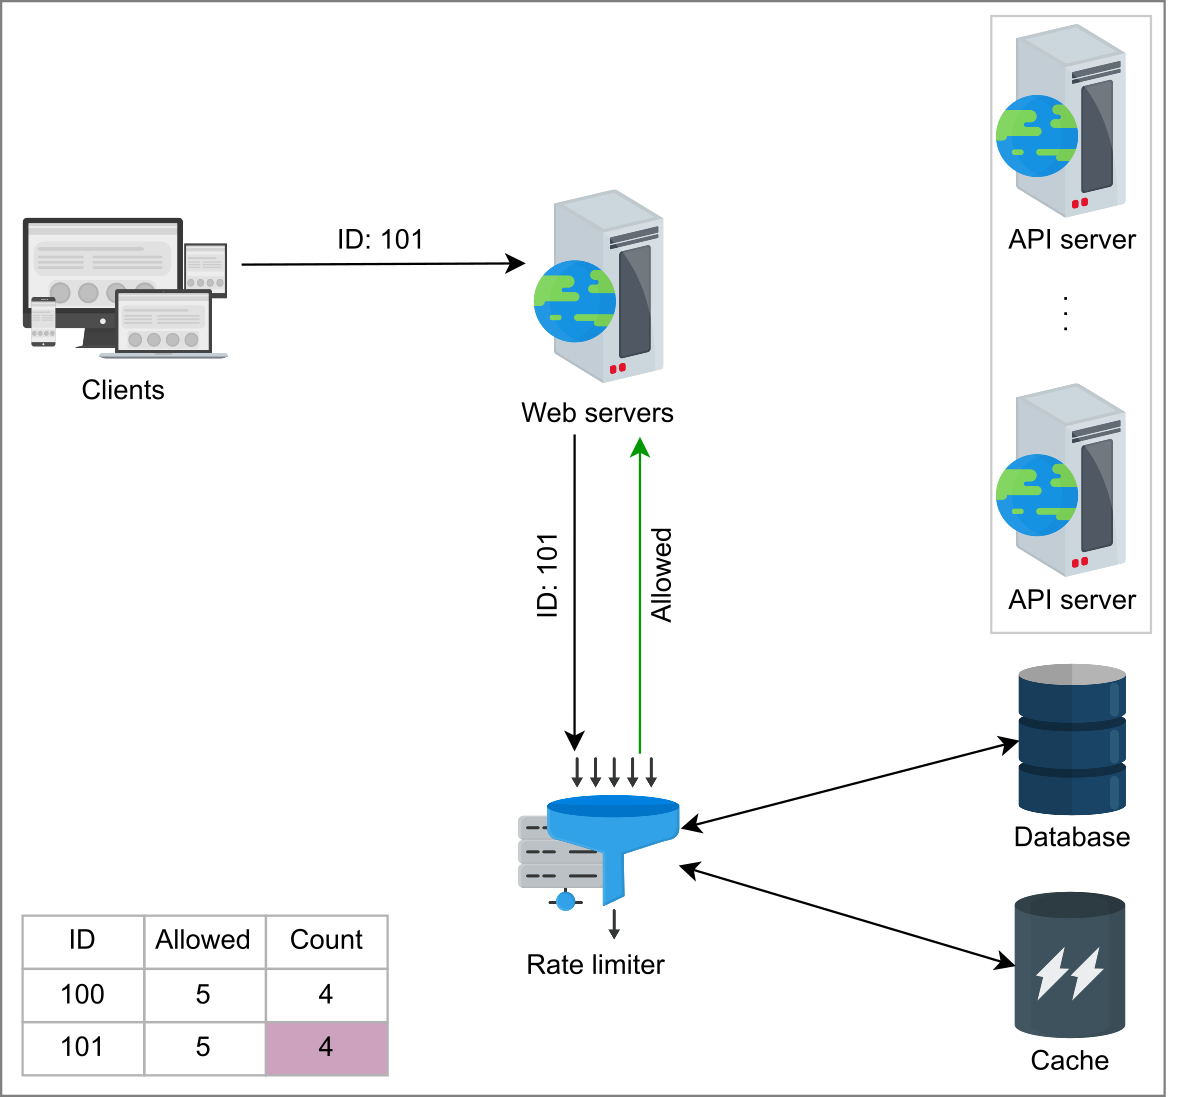
\includegraphics[width=\textwidth]{Images/chapter_19/section_5287353329647616/5073357414596608.png}
 \caption{If the request is allowed, the corresponding count is incremented}
 \end{subfigure}
 \hfill
 \begin{subfigure}[b]{0.48\textwidth}
 \centering
 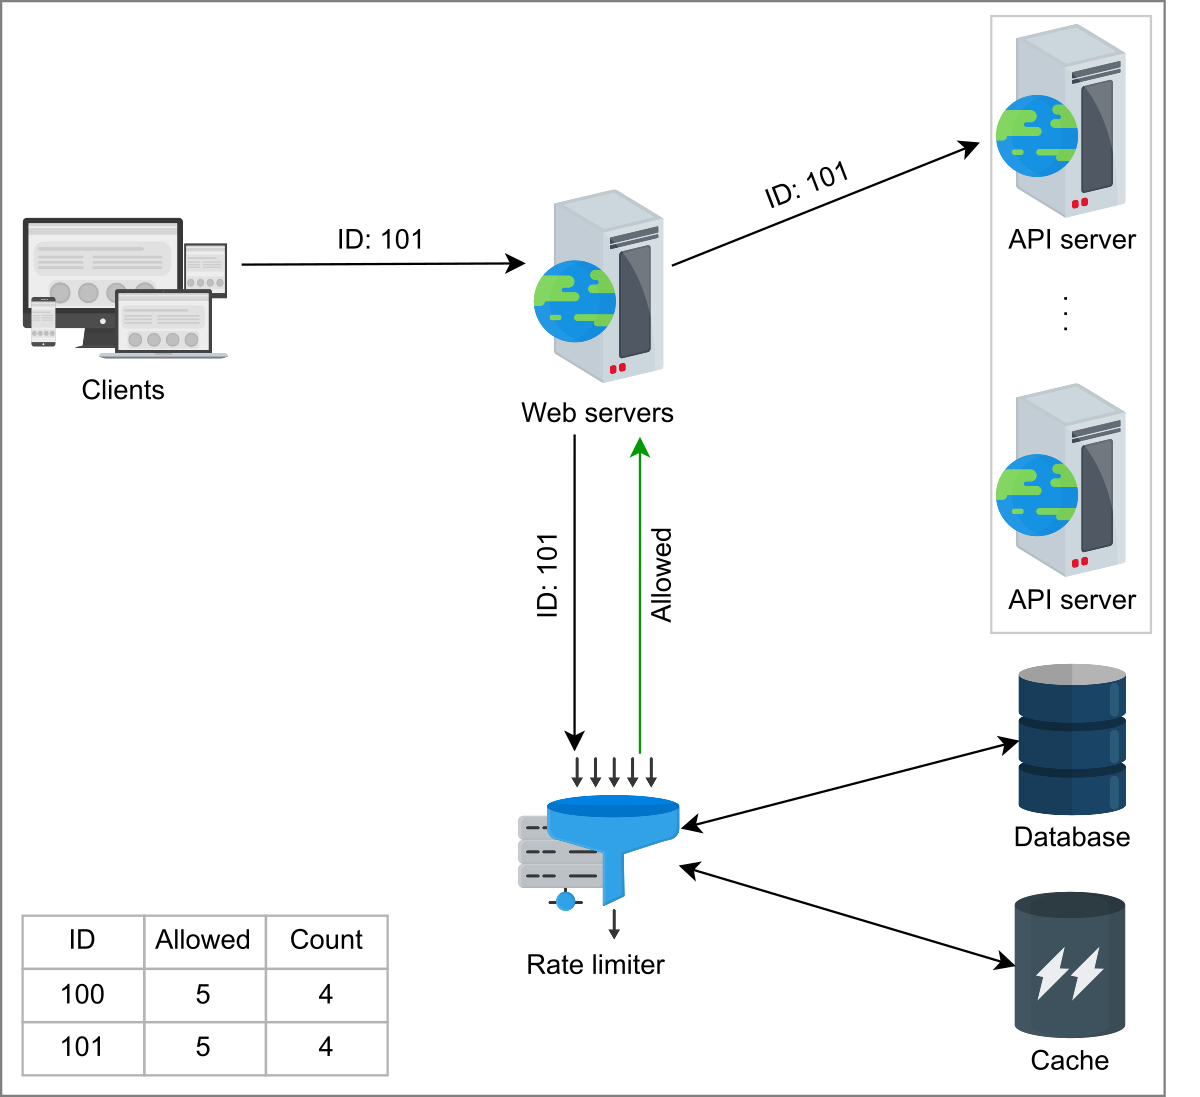
\includegraphics[width=\textwidth]{Images/chapter_19/section_5287353329647616/4862798463238144.png}
 \caption{The web server forwards the request to one of the API servers}
 \end{subfigure}
\end{figure}

\begin{figure}[htbp]
 \centering
 \begin{subfigure}[b]{0.48\textwidth}
 \centering
 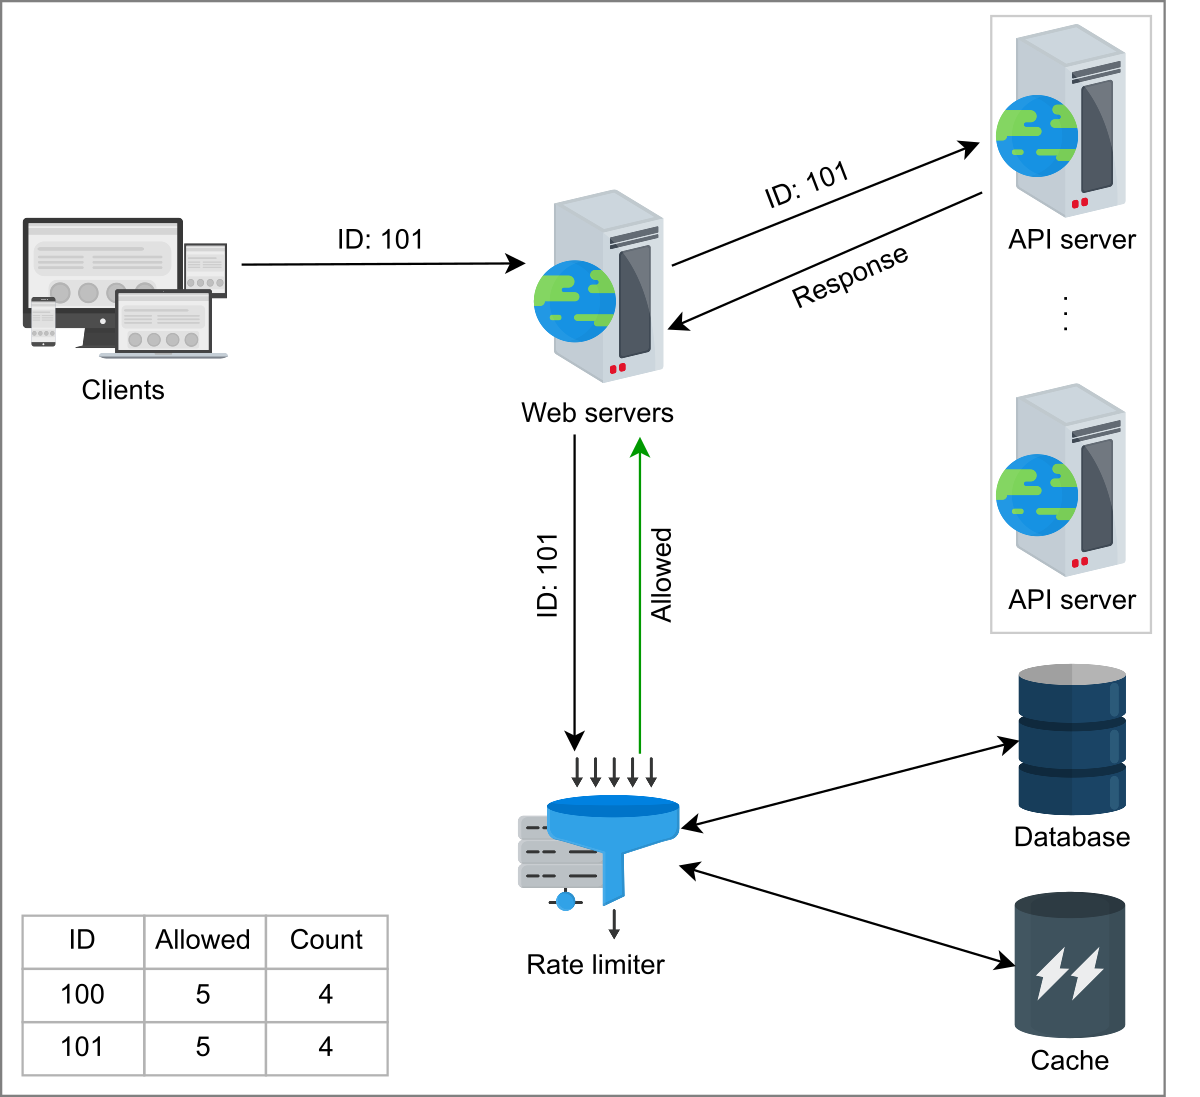
\includegraphics[width=\textwidth]{Images/chapter_19/section_5287353329647616/4864767126929408.png}
 \caption{The response is sent back to the web server after serving the request}
 \end{subfigure}
 \hfill
 \begin{subfigure}[b]{0.48\textwidth}
 \centering
 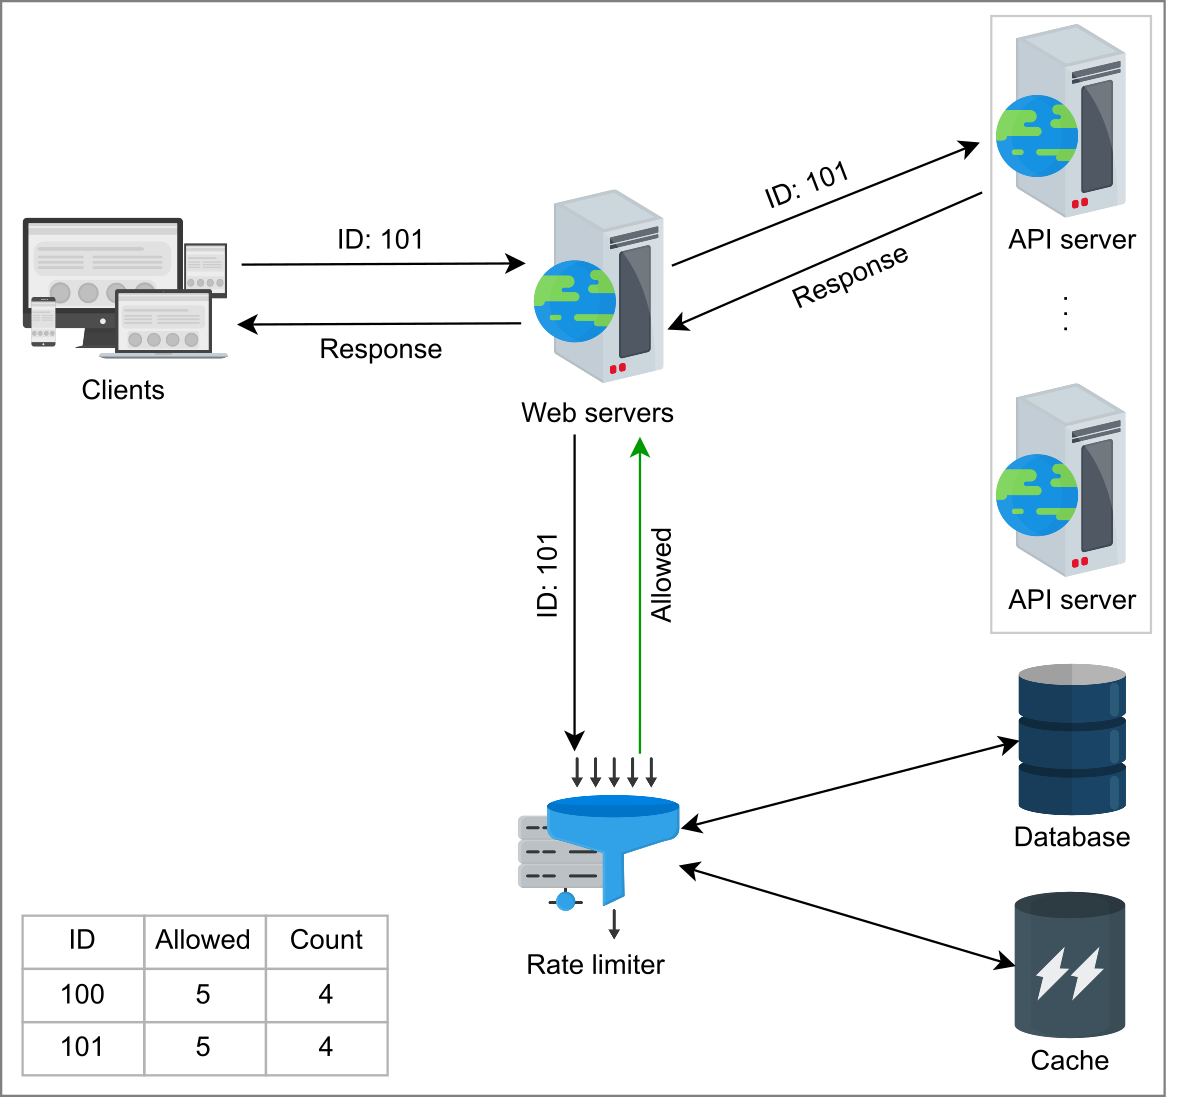
\includegraphics[width=\textwidth]{Images/chapter_19/section_5287353329647616/4900450050768896.png}
 \caption{Web server send the response back to the corresponding client }
 \end{subfigure}
\end{figure}

\subsection{Detailed design}\label{ca5wAS7jtdmGkmF9le_u6}
\\
The high-level design given above does not answer the following questions:

\begin{itemize}
\item
\protect\phantomsection\label{XBj5LDei_7GJdcbQFetsD}
Where are the rules stored?
\item
\protect\phantomsection\label{SkpbZfPVPgbI5wPHE9s_E}
How do we handle requests that are rate limited?
\end{itemize}
\\
In this section, we'll first expand the high-level architecture into several other essential components. We 'll also explain each component in detail, as shown in the following figure.

\begin{figure}[htbp]
 \centering
 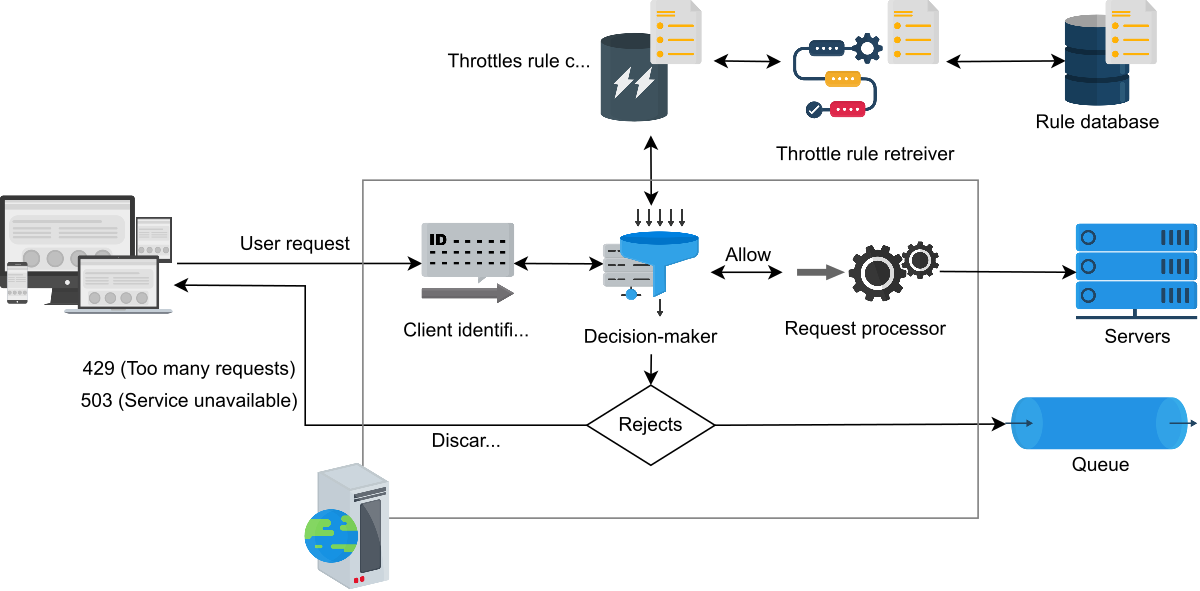
\includegraphics[width=0.5\textwidth]{Images/chapter_19/section_5287353329647616/4907692214976512.png}
 \caption{The rate limiter accepts or rejects requests based on throttle rules}
\end{figure}

Let's discuss each component that is present in the detailed design of a rate limiter.

\begin{itemize}
\item
\protect\phantomsection\label{JNj8RTMMm7X6jZZP2Y_Md}
\textbf{Rule database}: This is the database, consisting of rules defined by the service owner. Each rule specifies the number of requests allowed for a particular client per unit of time.
\item
\protect\phantomsection\label{PRflNHAtzykFINhzoxO-o}
\textbf{Rules retriever}: This is a background process that periodically checks for any modifications to the rules in the database. The rule cache is updated if there are any modifications made to the existing rules.
\item
\protect\phantomsection\label{_xV3XxmnaaEAPavRVHEu5}
\textbf{Throttle rules cache}: The cache consists of rules retrieved from the \textbf{rule database}. The cache serves a rate-limiter request faster than persistent storage. As a result, it increases the performance of the system. So, when the rate limiter receives a request against an ID (key), it checks the ID against the rules in the cache.
\item
\protect\phantomsection\label{o7CdlhVLejaortLmJD0n9}
\textbf{Decision-maker}: This component is responsible for making decisions against the rules in the cache. This component works based on one of the rate-limiting algorithms that are discussed in the next lesson.
\item
\protect\phantomsection\label{2_vqaDtyG94m1LTGXnA_B}
\textbf{Client identifier builder}: This component generates a unique ID for a request received from a client. This could be a remote IP address, login ID, or a combination of several other attributes, due to which a sequencer can't be used here. This ID is considered as a key to store the user data in the key-value database. So, this key is passed to the \textbf{decision-maker} for further service decisions.
\end{itemize}
\\
In case the predefined limit is crossed, APIs return an HTTP response code 429\ Too\ Many\ Requests, and one of the following strategies is applied to the request:

\begin{itemize}
\item
\protect\phantomsection\label{ZalF_f3XOX5G6fnxP1a8j}
Drop the request and return a specific response to the client, such as ``too many requests'' or ``service unavailable.''
\item
\protect\phantomsection\label{Ly4dwUxsRWLh0zkRPqehP}
If some requests are rate limited due to a system overload, we can keep those requests in a queue to be processed later.
\end{itemize}

\subsubsection{Request processing}\label{Q6MwqZQbCka7E0UBXLic7}
\\
When a request is received, the \emph{client identifier builder} identifies the request and forwards it to the \emph{decision-maker}. The decision-maker determines the services required by request, then checks the cache against the number of requests allowed, as well as the rules provided by the service owner. If the request does not exceed the count limit, it is forwarded to the \emph{request processor}, which is responsible for serving the request.
\\
The decision-maker takes decisions based on the throttling algorithms. The throttling can be hard, soft, or elastic. Based on \textbf{soft or elastic throttling}, requests are allowed more than the defined limit. These requests are either served or kept in the queue and served later, upon the availability of resources. Similarly, if \textbf{hard throttling} is used, requests are rejected, and a response error is sent back to the client.

\begin{center}\rule{0.5\linewidth}{0.5pt}\end{center}
\\
In the event of a failure, a rate limiter is unable to perform the task of throttling. In these scenarios, should the request be \textbf{accepted} \textbf{or} \textbf{rejected}?\\
\strut \\
Give your answer along with proper reasoning in the AI assessment widget below.

\textbf{Question:}

Should requests be rejected or accepted in face of failures?

\textbf{Reference Answer:}

Accepted. Because of the following reasons: Reason 1: In such a scenario, the proposed system should adhere to the non-functional requirements, including availability and fault tolerance. Reason 2: The decision would be not to throttle requests as we would have many rate limiters at different service levels. Reason
3: Even if there is no other rate limiter, the load balancer performs the task at a certain level.
\\
The engineering team should act quickly to resolve the failure, as it is a critical component in a system's infrastructure.

\subsubsection{Race condition}\label{TklBDgZ5IQh16oZ2EyK8T}
\\
There is a possibility of a race condition in a situation of high concurrency request patterns. It happens when the ``get-then-set'' approach is followed, wherein the current counter is retrieved, incremented, and then pushed back to the database. While following this approach, some additional requests can come through that could leave the incremented counter invalid. This allows a client to send a very high rate of requests, bypassing the rate-limiting controls. To avoid this problem, the locking mechanism can be used, where one process can update the counter at a time while others wait for the lock to be released. Since this approach can cause a potential bottleneck, it significantly degrades performance and does not scale well.
\\
Another method that could be used is the ``set-then-get'' approach, wherein a value is incremented in a very performant fashion, avoiding the locking approach. This approach works if there's minimum contention. However, one might use other approaches where the allowed quota is divided into multiple places and divide the load on them, or use sharded counters to scale an approach.
\begin{quote}
\textbf{Note:} We can use sharded counters for rate-limiting under the highly concurrent nature of traffic. By increasing the number of shards, we reduce write contention. Since we have to collect counters from all shards, our reading may slow down.
\end{quote}
\subsubsection{A rate limiter should not be on the client's critical path}\label{RoFeApY8UkdG-ip3TaCIH}
\\
Let's assume a real-time scenario where millions of requests hit the front-end servers. Each request will retrieve, update, and push back the count to the respective cache. After all these operations, the request is sent forward to be served. This approach could cause latency if there is a high number of requests. To avoid numerous computations in the client's critical path, we should divide the work into offline and online parts.
\\
Initially, when a client's request is received, the system will just check the respective count. If it is less than the maximum limit, the system will allow the client's request. In the second phase, the system updates the respective count and cache offline. For a few requests, this won't have any effect on the performance, but for millions of requests, this approach increases performance significantly.
\\
Let's understand the online and offline updates approach with an example. In the following set of illustrations, when a request is received, its ID is forwarded to the rate limiter that will check the condition if(request(ID). Count
\ \textless{=\ Max.\ Limit} by retrieving data from the cache. For simplicity, assume that one of the requests ID is 101, that is, request(ID)\ =\ 101. The following table shows the number of requests made by each client and the maximum number of requests per unit time that a client can make.

\begin{table}[htbp]
\centering
\small
\adjustbox{max width=\textwidth}{
\begin{tabular}{|p{0.367\textwidth}|p{0.320\textwidth}|p{0.263\textwidth}|}
\hline
Request ID & Maximum Limit & Count \\
\hline
\hline
100 & 5 & 4 \\
\hline
101 & 5 & 3 \\
\hline
\end{tabular}
}
\end{table}

If the condition is true, the rate limiter will first respond back to the front-end server with an \texttt{Allowed} signal. The corresponding \texttt{count} and other relevant information are updated offline in the next steps. The rate limiter writes back the updated data in the cache. Following this approach reduces latency and avoids the contention that incoming requests could have caused.

\begin{figure}[htbp]
 \centering
 \begin{subfigure}[b]{0.48\textwidth}
 \centering
 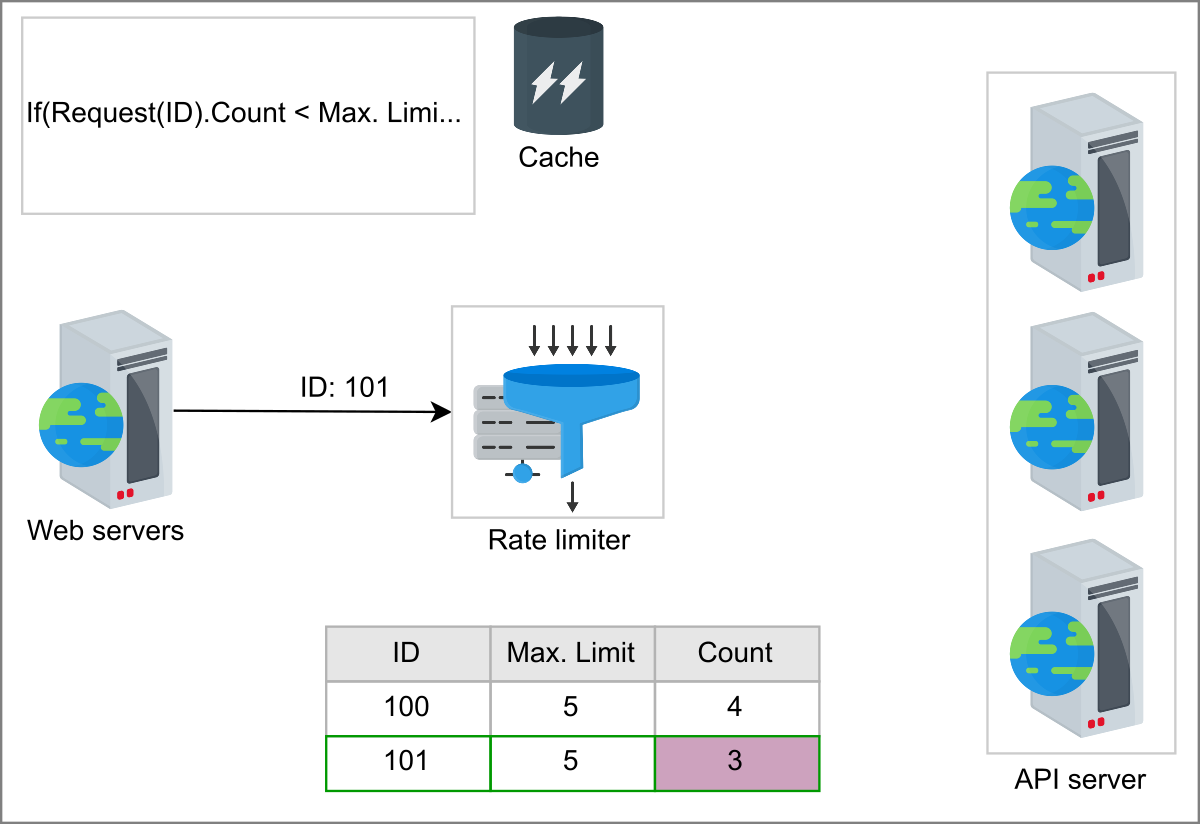
\includegraphics[width=\textwidth]{Images/chapter_19/section_5287353329647616/5137970600607744.png}
 \caption{A request with ID:101 is received. The count for this is 3 }
 \end{subfigure}
 \hfill
 \begin{subfigure}[b]{0.48\textwidth}
 \centering
 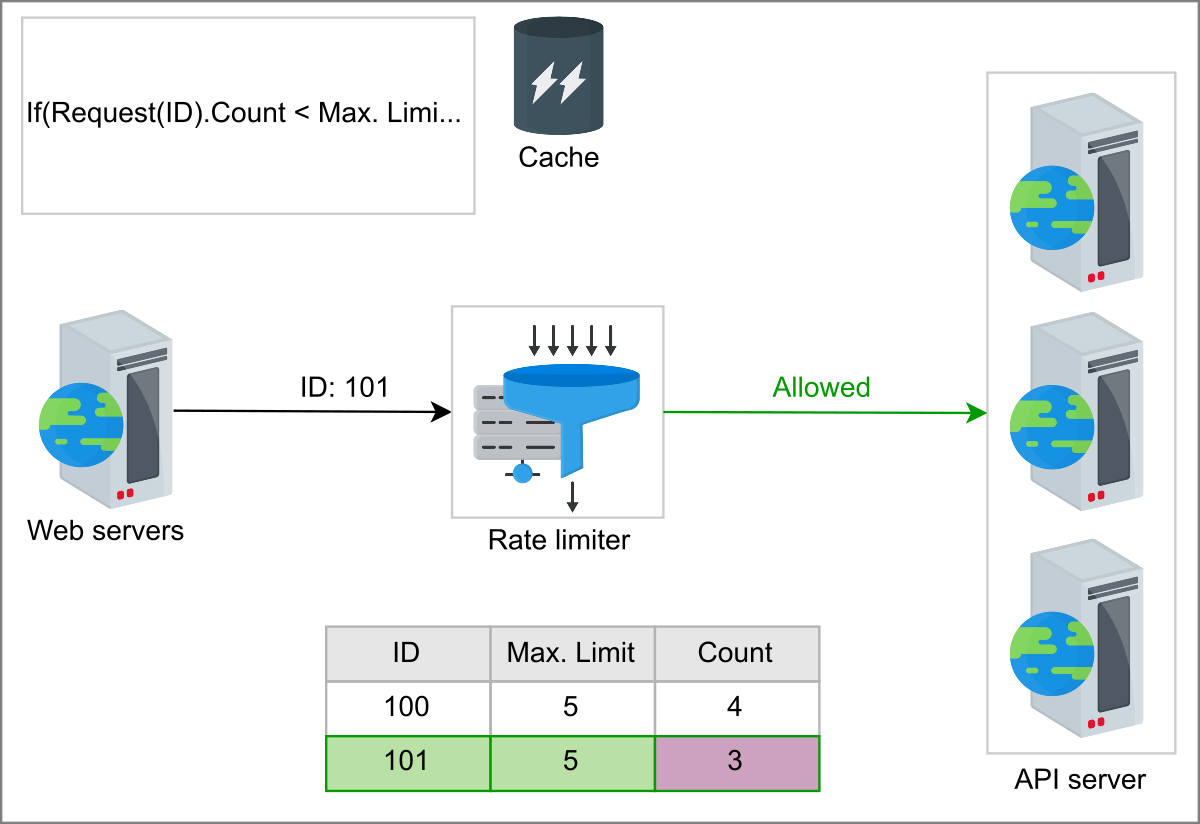
\includegraphics[width=\textwidth]{Images/chapter_19/section_5287353329647616/5415875452862464.png}
 \caption{The request is allowed, since 3 is less than 5 for ID 101}
 \end{subfigure}
\end{figure}

\begin{figure}[htbp]
 \centering
 \begin{subfigure}[b]{0.48\textwidth}
 \centering
 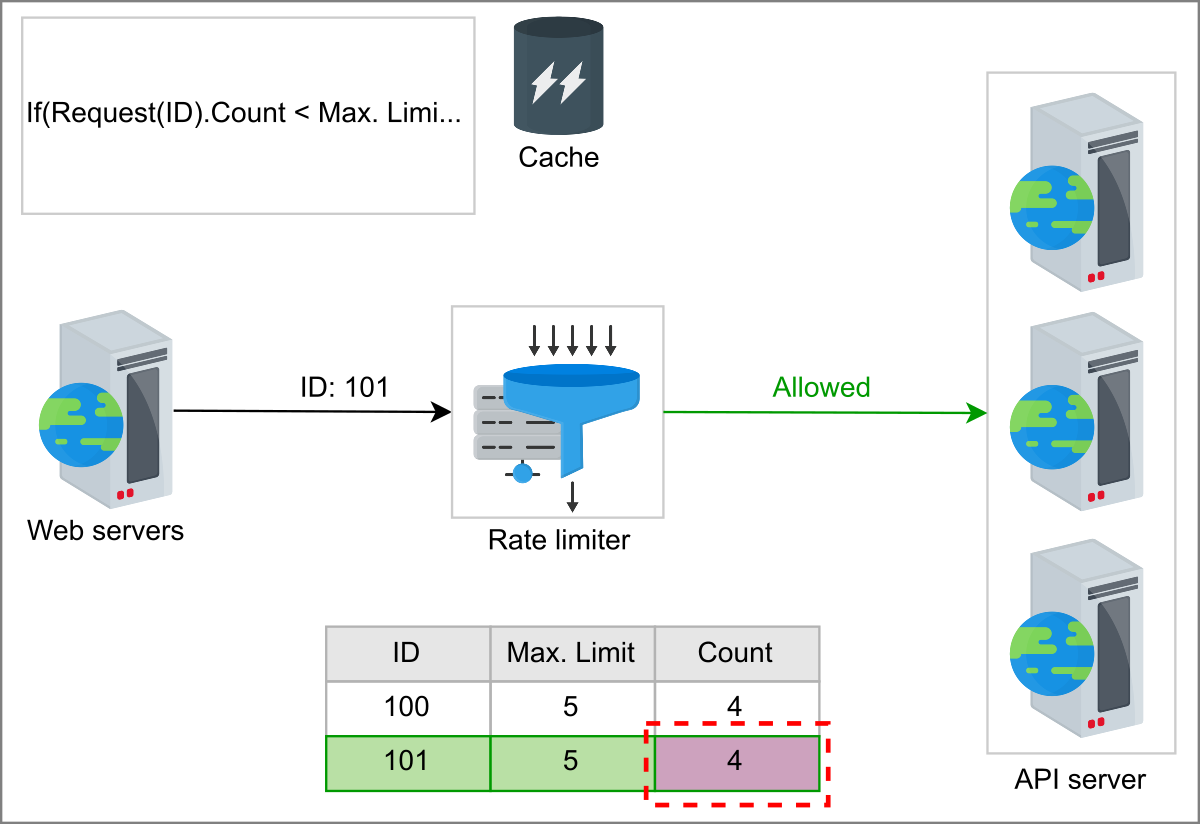
\includegraphics[width=\textwidth]{Images/chapter_19/section_5287353329647616/5411048647819264.png}
 \caption{In the next step, the Count and other relevant data is updated for the client with ID 101}
 \end{subfigure}
 \hfill
 \begin{subfigure}[b]{0.48\textwidth}
 \centering
 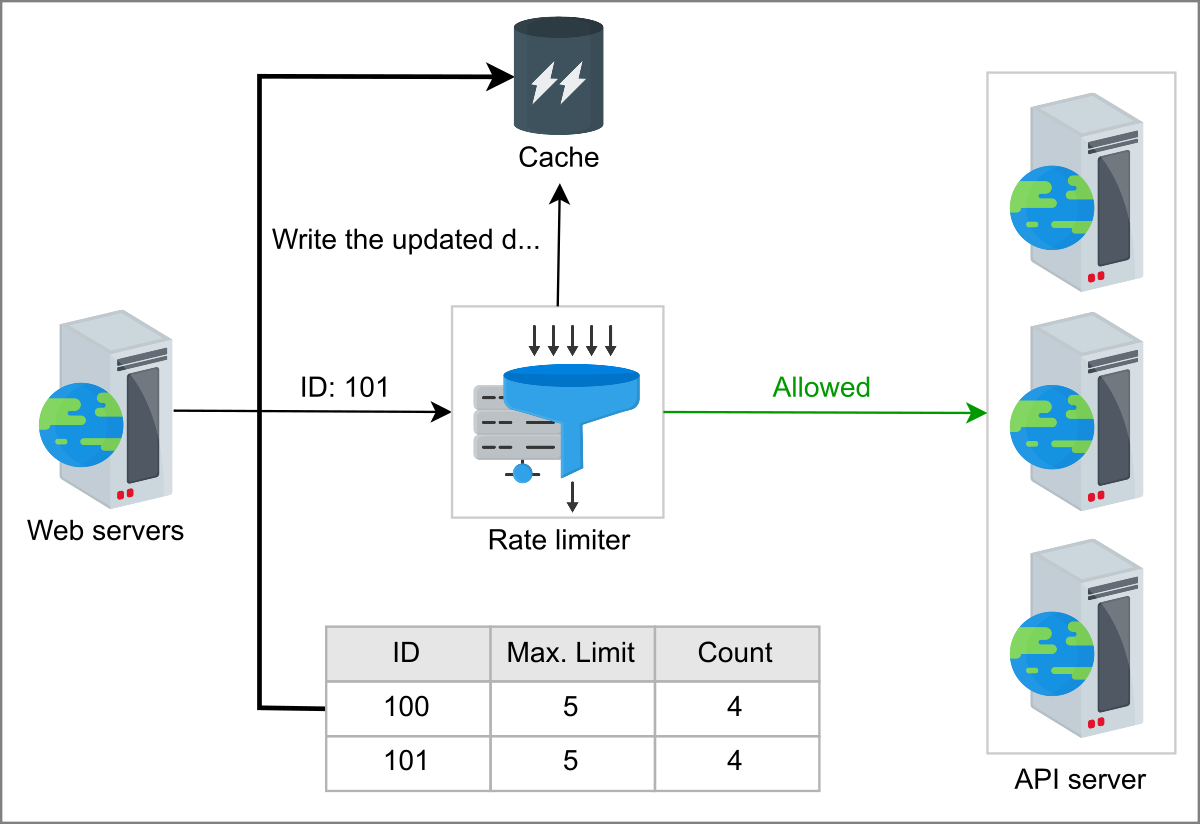
\includegraphics[width=\textwidth]{Images/chapter_19/section_5287353329647616/5387273294315520.png}
 \caption{After specific intervals the data is written back to the cache}
 \end{subfigure}
\end{figure}

\begin{quote}
\textbf{Note:} We've seen a form of rate limiting in TCP network protocol, where the recipient can throttle the sender by advertising the size of the window (the outstanding data a recipient is willing to receive). The sender sends the minimum value of either the congestion window or the advertised window. Many network traffic shapers use similar mechanisms to provide preferential treatment to different network flows.
\end{quote}
\subsection{Conclusion}\label{pPfrXbCLJbek-EUm5UBQ4}
\\
In this lesson, we discussed the design of a rate limiter in distributed systems. Let 's analyze the non-functional requirements we promised in the previous lesson.

\begin{itemize}
\item
\protect\phantomsection\label{RZvcuT9UPu8wldABAjjqw}
\textbf{Availability:} If a rate limiter fails, multiple rate limiters will be available to handle the incoming requests. So, a single point of failure is eliminated.
\item
\protect\phantomsection\label{itDDg_5Gkas7C-reFyto8}
\textbf{Low latency:} Our system retrieves and updates the data of each incoming request from the cache instead of the database. First, the incoming requests are forwarded if they do not exceed the rate limit, and then the cache and database are updated.
\item
\protect\phantomsection\label{_Uxqb8o5hAvJCuCLRBaKa}
\textbf{Scalability:} The number of rate limiters can be increased or decreased based on the number of incoming requests within the defined limit.
\end{itemize}
\\
Now, our system provides high availability, low latency, and scalability in light of the above discussion.

% End of section content